
Klasa \sokarclass{DicomScene} jest klasą abstrakcyjną i nie generuje obrazu, pozostawia do klasą dziedziczących po niej.

\paragraph{Cykl generowania obrazu}

Klasa \sokarclass{DicomScene} dostarcza następujące obiekty do generowania obrazu:
\begin{itemize}
    \item \cppcode{QMutex processing} mutex do zablokowania podczas generowania obrazu, aby parametry obrazu nie mogły być zmienianie podczas jego generowania.
    
    \item \cppcode{uint imgDimX} szerokość obrazu w pikselach.
    
    \item \cppcode{uint imgDimY} wysokość obrazu w pikselach.
    
    \item \cppcode{std::vector<Pixel> targetBuffer} wektor docelowego obrazu RGB o długości $imgDimX*imgDimY$.
    
    \cppcode{Pixel} to struktura reprezentujące piksel, wyglądające następująco:
    
    \cppcode{struct Pixel \{ quint8 red = 0, green = 0, blue = 0; \};}

    \item \cppcode{std::vector<char> originBuffer} wektor danych wypełniona danymi z jednej ramki o długośći iloczynu $imgDimX*imgDimY$ i ilości bajtów jednego piksela obrazu. 

    \item \cppcode{QImage qImage} obiekt obrazu.
    
    \qtclass{QImage} można zrobić z istniejącego bufora, w tym przypadku jest to \cppcode{targetBuffer}.
    Format obrazu to \qtclass{QImage::Format\_RGB888}, czyli trzy bajty, każdy na jeden kanał.

    \item \cppcode{QPixmap pixmap} obiekt obrazu do wyświetlania.
    
    Obiektów klasy \qtclass{QImage} nie da się wyświetlić, nie jest on przystosowany do wyświetlania.
    Natomiast klasa \qtclass{QPixmap} to reprezentacja obrazu dostosowana do wyświetlania ekranie, która może być używana jako urządzenie do malowania w bibliotece Qt.

    \item \cppcode{QPixmap iconPixmap} obiekt obrazu ikonu, docelowo powinien mieć 128 pikseli na 128 pikseli.
    
    \item \cppcode{QGraphicsPixmapItem *pixmapItem} wskaźnik do obiektu na scenie, który wyświetla \cppcode{pixmap}.
    
\end{itemize}

Generowanie obrazu jest robione przez funkcje \sokarclass{DicomScene::generatePixmap()}.
Po wywołaniu funkcji obiekt \cppcode{pixmap} powinien zawierać obraz wygenerowany z obecnymi parametrami.
Funkcja zwraca również \cppcode{bool}, który informuje nas czy \cppcode{pixmap} rzeczywiście został zmieniony.

Całe odświeżanie obrazu jest implementowane w funkcji \sokarclass{DicomScene::reloadPixmap()}.
Funkcja wywołuje \sokarclass{DicomScene::generatePixmap()} i odświeża \cppcode{pixmapItem} kiedy zajdzie taka potrzeba

Generowanie poszczególnych typów obrazów jest wyjaśnione poniżej.

\subsubsection{Monochorme}

Obraz monochromatyczny to obraz w odcieniach szarości, od białego do czarnego lub od czarnego do białego. Dane są zapisane w sposób ciągły wartość po wartości.

\paragraph{Zamysł generowania obrazu}

Mamy obraz, którego piksele to n-bitowe liczby, na przykład 16 bitowa liczba całkowita.
W takiej postaci wyświetlemoe obrazu na monitorze RGB lub nawet na profesjonalnym 10-bitowym jest niemożliwe.
Należy taką liczbę przerobić na trzy liczby, reprezentujące 3 kanały RGB, czerwony, zielony i niebieski.
Dlatego do wyświetlania obrazów monochromatycznych o dużym kontraście stosuję się twór zwany okienkiem.
Jest to funkcja która mapuje n-bitwy obraz na 8-bitowy obraz w skali szarości.
8-bitów, ponieważ monitor RGB jest wstanie wyświetlić 256 odcieni szarości.

\subparagraph{Wyznaczanie okiena}
Przyjeło się, że okienko definiuje się dwoma liczbami: środkiem, oznaczanym jako $center$ i długością, oznaczaną jako $width$.
Wyznaczamy zakres okienka $x_0$ i $x_1$ z środka okienka $center$ i długości $width$.
\[x_0 = center - width / 2\]
\[x_1 = center + width / 2\]
Wyznaczamy parametry $a$ i $b$, prostej przechodzącej przez dwa punkty $(x_0, y_0)$ i $(x_1, y,_1)$.
Gdzie $y_0$ jest równe 0, a $y_1$ jest równe 255.
Funkcja okienka wygląda następująco:
\[
    f(v)=
    \begin{cases}
        0     & \text{gdy $0 \le v \wedge v \le x_0$ } \\
        a*x+b & \text{gdy $x_0 < v \wedge v < x_1$}    \\
        255   & \text{gdy $x_1 \le v \wedge v \le 1$ }
    \end{cases}
\]

gdzie $v$ to wartość piksela danych obrazu.

Następnie przepuszczamy cały obraz przez funkcje okienka i otrzymujemy obraz w skali od $0$ do $255$.
Taki odraz w skali od można już wyświetlić.
Natomiast standard DICOM przewiduje, że obraz można jeszcze wyświetlić w wielokolorowej palecie barw.
Przykład takiej palety HotIron w porównaniu do skali szarości można zobaczyć na rysunku .
Taka paleta barw nie koniecznie musi mieć 256 odcieni, dlatego lepiej jest zrobić aby okienko, mapowało na liczbę od 0 do 1, a później paleta mapowała na kolor RGB.

\begin{figure}[!htbp]
    \centering
    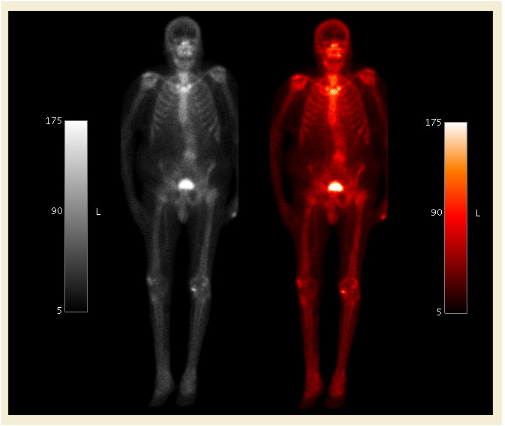
\includegraphics[width=0.7\textwidth]{img/monochrome-001.png}
    \caption{Paleta HotIron w porównaniu do palety w skali szarości}
    \label{fig:monochrome1}
\end{figure}

Teraz iterujemy po wszystkich możliwych wartościach wartośćiach obrazu i wykonujemy takie operacje.
\begin{itemize}
    \item wyznaczenie wartości okienka.
          \[y = a * x + b\]
    \item y zostaje obcięcie do 1.0 lub 0.0 jeżeli wyjdzie poza zakres od 1.0 do 0.0
    \item pobranie z palety piksel odpowiadający wartości
    \item wsadzenie piksela do tablicy, tak aby najmniejsza wartości obrazu miała indeks 0 a największy ostani
\end{itemize}


\paragraph{Implementacja algorytmu}

\subparagraph{Opis}
\par
Implementacja powyżej przedstawionego algorytmu w sposób dosłowny byłaby mało optymalna dla maszyny i wymagała by wielu pobocznych tablic oraz względnie dużej ilości mnożenia.
Trzeba też zauważyć, że do wyliczenie jakiegoś piksela nie potrzeba liczyć, żadnego innego piksela, co skutkuje, że każdy piksel można wyliczyć oddzielnie.
Dlatego najlepiej było by współbieżnie przelecieć po całym obrazie i zamienić dane na piksele.
Ale do zamiany dane na piksel, musimy mnożyć i dzielić liczby zmiennoprzecinkowe, a to do najszybszych nie należy.
Dlatego dobrym pomysłem jest zrobienie mniejszej tablicy typu LookUpTable, wypełnienie jej wszystkimi możliwymi wartościami obrazu, a następnie przerobić obraz z tablicą LUT.
Ale ponieważ tablica LUT posiada wszystkie możliwe kombinacje wartości, jej rozmiar można wyznaczyć wzorem: $2^N*3$, gdzie N to liczba bitów liczby.
Standard DICOM definiuje, że liczby mogą mieć $8$, $12$, $16$, $32$ i $64$ bity, jednakże, $12$ bitowe i tak się zapisuje w postaci 16-bitowych w pamięci RAM.
Dlatego możliwe wartości wielkości tablicy LUT to w przybliżeniu: $768$ bajtów, $196$ kilobajtów, $12,5$ gigabajtów i $56$ eksabajta($55*10^{6}$ terabajtów).
Alokowanie dwóch największych wartości może być lekko problematyczne, dlatego zrobiłem dwie implementacje algorytmu: z tablicą LUT(dla 8 i 16 bitowych obrazów i bez tablicy LUT(dla 32 i 64 bitowych obrazów).
Algorytm składa się z 3 części: wyznaczenie parametrów okna, przygotowanie okna (tylko gdy jest tablica LUT), wielowątkowa iteracja po obrazie.
\par
Okno z LUT jest implementowane przez \sokarclass{Monochrome}{WindowIntDynamic}.
Okno bez LUT jest implementowane przez \sokarclass{Monochrome}{WindowIntDynamic}.
Obie klasy dzidziczą po abstrakcyjnej klasie \sokarclass{Monochrome}{Window}m, która z kolei dziedziczy po \sokarclass{SceneIndicator}, dlatego od razu może wyświetlać obecne wartości okna.
\par
UWAGA: Standard DICOM zakłada, że danymi mogą być liczby całkowite(\cppcode{int}) oraz zmiennoprzecinkowe(\cppcode{float} lub \cppcode{double}), ale praktycznie, nie ma takich aparatów medycznych, które zapisywały by takie obrazy, gdzie dane to liczby zmiennoprzecinkowe. Dlatego założyłem, że takie obrazy nie istnieją.

\subparagraph{Wyznaczenie parametrów okna}
\par
Najpierw wyznaczam okienko, które zmienia wartości obrazu na skale od zera do jeden:
\[x_0 = center - width / 2\]
\[x_1 = center + width / 2\]
\[y_1 = 0.0\]
\[y_0 = 1.0\]
gdzie:
\begin{itemize}
    \item $center$ --- środek okienka
    \item $width$ --- szerokość okienka
    \item $x0$ i $y0$ --- współrzędne pierwszego punktu
    \item $x1$ i $y1$ --- współrzędne drugego punktu
\end{itemize}
Przeglądarka pozwala na inwersje okienka.
Dlatego kiedy użytkownik zażyczy sobie inwersji, zmienne $y0$ i $y1$ zamienią się wartoścami.

Standard DICOM przewiduje, że wszystkie dane powinny być wyskalowane, za pomocą wzoru.
\[OutputUnits = m*SV + b\]
gdzie:
\begin{itemize}
    \item $m$ --- wartość z \dicomtag{RescaleSlope}{0028}{1053}
    \item $b$ --- wartość z \dicomtag{RescaleIntercept}{0028}{1052}
    \item $SV$ --- stored values - warość pixela z pliku
    \item $OutputUnits$ --- wartość wynikowa
\end{itemize}

Wartości okienka odnoszą się do wartości już wyskalowanej, a ponieważ skalowanie całego obrazu jest czasochłonne, przeskalowaie okienka da taki sam efekt:
\[(OutputUnits - b ) / m = SV \]
więc:
\[x_0 -= rescaleIntercept\]
\[x_1 -= rescaleIntercept\]
\[x_0 /= rescaleSlope\]
\[x_1 /= rescaleSlope\]

Posiadamy, teraz dwa punkty okienka odnoszące się do wartośći obrazu.
Wyznaczam parametry prostej przechodzącej przez dwa punkty:
\[a = (y_1 - y_0) / (x_1 - x_0)\]
\[b = y_1 - a * x_1\]

\par
Teraz algorytm się rozdwaja.
Pobieranie wartości z okienka odbywa się za pomocą funkcji \sokarclass{Monochrome}{Window\zerospace::{\zerospace}getPixel()}.


\subparagraph{Implementacja dynamiczna bez tablicy LUT}

\par
W tej wersji funkcja \sokarclass{Monochrome}{Window\zerospace::{\zerospace}getPixel()}wygląda następująco:
\par
NAUCZYĆ SIĘ WSTAWIAĆ KOD C++
\par
Widzimy tutaj, że funkcja najperw sprawdza czy zakres okienka został przekroczony, następnie wylicza wartość obrazu i pobiera kolor z palety.
\par
UWAGA: ponieważ nie dysponuje rzeczywistym obrazem o pikselu danych 32-bitowym lub 64-bitowych, implementacja dynamiczna nie była testowana w warunkach rzeczywistych.

\subparagraph{Implementacja statyczna z tablicą LUT}

\subparagraph{Iterowanie po obrazie}

\paragraph{Palety}
Klasa \sokarclass{Palette} reprezentuje palety kolorów używanych do kolorowania obrazu monochromatycznego.
Paleta przerabia liczbę zmiennoprzecinkową od zera do jedynki na kolor RGB, zwracając \sokarclass{Pixel}.
Palety są wczytywane z plików XML i można definiować własne palety z poza standardem.



\subsubsection{RGB}

Obrazów zapisanych w RGB nie trzeba w żaden sposób obrabiać, dane już są prawie gotowe do wyświetlenia, należy je tylko odpowiednio posortować, tak jak wymaga biblioteka QT.
Sposób posortowania wartości w pilku określa \dicomtag{PlanarConfiguration}{0x0028}{0006}. Może o przyjąć dwie następujące wartośći:

\begin{itemize}
    \item 0 - oznacza to, że wartości pikseli są ułożone w taki sposób
        \[R1, G1, B1, R2, G2, B2, R3, G3, B3, R4, G4, B4,  ...\]
    \item 1 - oznacza to, że wartości pikseli są ułożone w taki sposób
        \[R1, R2, R3, R4, ... , G1, G2, G3, G4, ..., B1, B2, B3, B4, ...\]
\end{itemize}
gdzie:
\begin{itemize}
    \item Rn --- wartość czerwonego kanału
    \item Gn --- wartość zielonego kanału
    \item Bn --- wartość niebieskiego kanału
\end{itemize}

Wartości obrazu są przepisywane do bufora dla biblioteki QT.


\subsubsection{YBR}
Skórt YBR odpowiada skrótowi YCbCr.
Wartości są ułożone w taki sposób.
\[Y1, B1, R1, Y2, B2, R2, Y3, B3, R3, Y4, B4, R4,  ...\]

Ponieważ wartości te reprezentują kolory, są już w pewnym sensie są obrazem, ale nie można go wyświetlić, ponieważ komputery bazują na kolorach RGB.
Dlatego odpowieni algorytm konwertuje kolor YBR na kolor RGB, iterując po wszystkich wartościach obrazu.

\paragraph{Konwersja koloru YBR na kolor RGB}

YBR albo YCbCr to model przestrzeni kolorów do przechowywania obrazów i wideo.
Wykorzystuje do tego trzy typy danych: Y – składową luminancji, B lub Cb – składową różnicową chrominancji Y-B, stanowiącą różnicę między luminancją a niebieskim, oraz R lub Cr – składową chrominancji Y-R, stanowiącą różnicę między luminancją a czerwonym.
Kolor zielony jest uzyskiwany na podstawie tych trzech wartości.
YBR nie pokrywa w całości RGB, tak jak RGB nie pokrywa YBR.
Posiadają one część wspólną, co uniemożliwia wyświetlenie obrazu w stu procentach bez zniekształceń.
